\documentclass[pdf, handout]{beamer} % Add the [handout] option to group all of the items
\usetheme{Copenhagen}
\setbeamertemplate{theorems}[numbered]


\usepackage{amsthm}
\usepackage{amsmath}
%\setbeameroption{show notes on second screen=right}
%\setbeameroption{show only notes}
\usepackage[utf8]{inputenc}
\usepackage[spanish]{babel}
\usepackage[inference]{semantic}
\usepackage{tabularx}

\uselanguage{Spanish}
\languagepath{Spanish}

\title{Formalización del sistema de permisos de Android 10}

\author[Universidad Nacional de Rosario]{Guido De Luca}
\institute{Universidad Nacional de Rosario}
\date{\today}

\subject{Tesina}


\begin{document}

\newcommand{\AppId}{\mathsf{AppId}}
\newcommand{\Manifest}{\mathsf{Manifest}}
\newcommand{\Cert}{\mathsf{Cert}}
\newcommand{\Res}{\mathsf{Res}}
\newcommand{\AndroidState}{\mathsf{AndroidST}}
\newcommand{\iComp}{\mathsf{iComp}}

\newcommand{\Action}{\mathsf{Action}}
\newcommand{\Intent}{\mathsf{Intent}}

\newcommand{\Perm}{\mathsf{Perm}}
\newcommand{\PermGrp}{\mathsf{PermGroup}}
\newcommand{\Dangerous}{\mathsf{dangerous}}
\newcommand{\Normal}{\mathsf{normal}}

\newcommand{\ap}[2]{\mbox{$\mathit{#1}(#2)$}}
\newcommand{\bap}[3]{\mbox{$\mathit{#1}(#2,#3)$}}
\newcommand{\step}[1]{\mathbin{\lower0.55ex\hbox{$\lhook\joinrel\xrightarrow{#1}$}}}
\newcommand{\semstep}[1]{\step{#1}}
\newcommand{\Mathexecrel}[3]{#1 \semstep{#2} #3}
\newtheorem{prop}{Propiedad}


\begin{frame}[plain]
    \titlepage
\end{frame}

\begin{frame}{Motivación}
    \begin{itemize}
        \item ¿Por qué Android? \pause Por su popularidad y alcance \pause
        \item ¿Por qué un sistema de permisos? \pause Mediador entre usuarios y aplicaciones \pause
        \item ¿Por qué métodos formales? \pause
              \begin{itemize}[<+->]
                  \item Pruebas rigurosas
                  \item Aclarar comportamientos ambiguos
                  \item Construir un framework para razonar sobre el sistema
              \end{itemize}
    \end{itemize}
\end{frame}

\begin{frame}{J.P. Anderson, 1972}
    Diseño de un mecanismo de validación por referencia:
    \pause
    \begin{itemize}[<+->]
        \item Mediación completa
        \item A prueba de manipulaciones
        \item Verificable
    \end{itemize}
\end{frame}


\begin{frame}{Un poco de contexto sobre Android}{Componentes del sistema}
    \begin{itemize}[<+->]
        \item \textbf{Actividad}: representa una pantalla individual con interfaz de usuario
        \item \textbf{Servicio}: realiza operaciones de ejecución prolongada en segundo plano
        \item \textbf{Receptor de emisiones}: permite que el sistema u otras aplicaciones entreguen
              mensajes por fuera del flujo normal
        \item \textbf{Proveedor de contenido}: administra los datos de una aplicación para que
              puedan ser compartidos con otras
    \end{itemize}
\end{frame}

\begin{frame}{Un poco de contexto sobre Android}{Interacción entre componentes}
    \textit{Intents:} \\
    \begin{itemize}
        \item Mensajería utilizada para la comunicación entre componentes \pause
        \item Puden ser explícitos o implícitos
    \end{itemize}
    \vspace{20px} \pause
    Para recibir \textit{intents} implícitos, las aplicaciones declaran filtros de \textit{intents}.
    Este filtro se define en el \textbf{manifiesto} de la aplicación.
\end{frame}

\begin{frame}{Un poco de contexto sobre Android}{Permisos}
    Los recursos de una aplicación se protegen con distintos niveles de permisos.
    \begin{itemize}[<+->]
        \item Normal
        \item Peligrosos
        \item De misma firma
    \end{itemize}
    \vspace{20px} \pause Los permisos peligrosos se  otorgan en tiempo de ejecución. El resto, al
    instalar la aplicación.

    \vspace{20px} \pause Los permisos que pertenecen a una misma característica de una aplicación
    se agrupan en lo que definimos \textbf{grupo de permisos.}
\end{frame}

\begin{frame}{Un poco de contexto sobre Android}{Cambios de comportamiento recientes I}
    \textbf{Sistema de archivos}\\
    \vspace{10px}
    \begin{itemize}
        \item Los directorios de las aplicaciones tienen permisos restringidos
        \item Evita la fuga de metadatos
        \item Utilizar el mecanismo de \textit{intents} como la única forma segura de compartir
              archivos
    \end{itemize}
    \vspace{10px}
    \pause
    Cambio introducido en Android 7.
\end{frame}

\begin{frame}{Un poco de contexto sobre Android}{Cambios de comportamiento recientes II}
    \textbf{Cambios en permisos agrupados} \\
    \vspace{10px}
    Antes de Android 8, al otorgar un permiso peligroso, se otorgaban de manera incorrecta el resto
    de los permisos del grupo.\\
    \vspace{5px}
    A partir de esta versión de Android se corrige ese comportamiento y se define una noción de
    ``otorgamiento automático'' para permisos peligrosos.

    \vspace{10px} \pause
    \textbf{Permisos normales y peligrosos compartiendo grupo} \\
    \begin{block}{}
        ``Cualquier permiso puede pertenecer a un grupo de permisos sin importar el nivel del
        protección del mismo''
    \end{block}
    \pause
    ¿Cómo se comporta el sistema en este caso?
\end{frame}

\begin{frame}{Un poco de contexto sobre Android}{Cambios de comportamiento recientes III}
    \textbf{Chequeo de permisos en aplicaciones viejas} \\
    \vspace{10px}
    Alerta al usuario ante la ejecución de una aplicación cuyos permisos peligrosos fueron otorgados
    en tiempo de instalación.
\end{frame}

\begin{frame}{Nuestra formalización del sistema de permisos}{Consideraciones generales I}
    Lenguaje formal utilizado: Coq
    \vspace{10px}
    \begin{block}{}
        Coq es un \textit{framework} que provee un lenguje formal para escribir definiciones
        matemáticas, algoritmos ejecutables y teoremas, junto con un entorno semi-interactivo para
        escribir demostraciones con la asistencia de una computadora.
    \end{block}
\end{frame}

\begin{frame}{Nuestra formalización del sistema de permisos}{Consideraciones generales II}
    Estado del modelo: parte estática y parte dinámica
    \begin{itemize}
        \item Agregamos al estado previo un registro de las aplicaciones \textit{legacy} verificadas
        \item Mantuvimos noción de estado válido
    \end{itemize}
    \pause \vspace{20px}
    Acciones del modelo:
    \begin{itemize}
        \item Representan operaciones reales de Android.
        \item En términos de nuestro modelo, son transiciones de estado.
        \item Su semántica está dada en términos de pre-condición y post-condición
    \end{itemize}
\end{frame}

\begin{frame}{Nuestra formalización del sistema de permisos}{Acciones I}
    \texttt{grant}\\
    \vspace{5px}
    Acción utilizada para otorgar permisos no agrupados o el primer permiso de un grupo en ser
    otorgado.\\
    \pause
    \vspace{10px}
    \texttt{grantAuto}\\
    \vspace{5px}
    Acción que simboliza el otorgamiento automático de permisos. La precondición se cumple solamente
    cuando el permiso está agrupado y cuando la aplicación ya cuenta con dicho grupo validado.
\end{frame}

\begin{frame}{Nuestra formalización del sistema de permisos}{Acciones II}
    \texttt{verifyOldApp}\\
    \vspace{5px}
    Modela el cambio introducido en Android 10 para re-chequear los permisos de las aplicaciones
    \textit{legacy}.
    \pause
    \vspace{10px}
    \texttt{receiveIntent}\\
    \vspace{5px}
    A partir de ahora, las aplicaciones \textit{legacy} podrán postularse para resolver
    \textit{intents} implícitos pero no podrán recibirlos si no fueron verificadas.
\end{frame}

\begin{frame}{Nuestra formalización del sistema de permisos}{Acciones III}
    \texttt{revoke} y \texttt{revokePermGroup}\\
    \vspace{5px}
    Estas acciones se modificaron para mantenerse alineadas con la experiencia de usuario:
    \texttt{revoke} revoca permisos no agrupados y \texttt{revokePermGroup} elimina todos los
    permisos pertenecientes a ese grupo.\\
\end{frame}


\begin{frame}{Nuestra formalización del sistema de permisos}{Ejecuciones}
    Definimos una noción de ejecución a partir de una sucesión de acciones.

    \begin{displaymath}
        \fontsize{8pt}{9pt}\selectfont
        \begin{array}{c}
            \inference[]{$$valid\_state(s)$$ \hspace{.2cm} $$Pre(s, a)$$ \hspace{.2cm} $$Post(s, a, s')$$}{$$s\step{a/ok}s'$$}
            \hspace{0.5cm}
            \inference[]{$$valid\_state(s)$$ \hspace{.2cm} $$ErrorMsg(s, a, ec)$$}{$$s\step{a/error(ec)}s$$}
        \end{array}
    \end{displaymath}
    \pause
    \begin{theorem}{Las ejecuciones preservan la validez del estado}
        \fontsize{9pt}{12pt}\selectfont
        $\begin{array}{l} \forall\ (s\ s':\AndroidState)(a:\Action) (r:Response), s\step{a/r}s'
                \rightarrow valid\_state(s')\end{array}$
    \end{theorem}
\end{frame}

\begin{frame}{Propiedades del modelo}
    Solo los permisos pertenecientes a grupos autorizados puede ser otorgados automáticamente.
    \pause \vspace{20px}
    \begin{prop} \mbox{} \\
        \fontsize{9pt}{15pt}\selectfont
        $\forall (s,s': \AndroidState) (p:\Perm) (g:\PermGrp) (app:\AppId),$ \\
        $getPermissionLevel(p) = dangerous\ \land$ \\
        $getPermissionGroup(p) = Some\ g\ \land$ \\
        $g \notin getAuthorizedGroups(app,s) \rightarrow\ \neg\ \Mathexecrel{s}{\texttt{grantAuto}~p~app/ok}{s'}$ \\
    \end{prop}
\end{frame}

\begin{frame}{Más propiedades del modelo}
    \begin{prop}
        Un permiso puede ser otorgado automáticamente a una aplicación, a pesar de que
        \textbf{actualmente} no existan otros permisos de ese mismo grupo ya otorgados a la misma
    \end{prop}
    \pause \vspace{20px}
    \begin{prop}
        Una aplicación que usa un permiso normal y uno peligroso del mismo grupo de permisos, puede
        obtener el segundo automáticamente luego de ser instalada.
    \end{prop}
\end{frame}

\begin{frame}{Y más propiedades del modelo}
    \begin{prop}
        Una aplicación vieja que no ha sido verificada por el usuario no está autorizada a recibir
        intents.
    \end{prop}
    \pause \vspace{20px}
    \begin{prop}
        Cuando un usuario revoca el acceso a un grupo de permisos para determinada aplicación, todos
        los permisos individuales son revocados también.
    \end{prop}
\end{frame}

\begin{frame}{Nuestra implementación del sistema de permisos}
    Actualizamos la implementación funcional certificada con respecto a nuestro modelo formal.
    \begin{itemize}
        \item Actualizar definiciones de funciones existentes
        \item Agregar funciones nuevas
    \end{itemize}
    \pause \vspace{20px}
    \begin{theorem}
        [Corrección de la implementación]
        $ \forall\ (s:\AndroidState)\ (a:\Action),$ \\
        $\quad \quad \ap{valid\_state}{s} \rightarrow\ s\step{a/step(s,a).resp} \bap{step}{s}{a}.st$
    \end{theorem}
\end{frame}

\begin{frame}{Propiedades de la implementación}
    \begin{prop}
        Si una aplicación vieja está en condiciones de ser ejecutada entonces \textbf{debe} haber
        sido verificada por el usuario previamente.
    \end{prop}

    \begin{prop}
        La única forma de que una aplicación consiga un permiso es si el usuario lo autoriza, o
        si el usuario había autorizado un grupo previamente y el sistema puede otorgar el permiso
        automáticamente.
    \end{prop}

    \begin{prop}
        Si un permiso fue revocado, solo volver a otorgarlo bajo la autorización del usuario
        permitirá que una aplicación vuelva a tenerlo.
    \end{prop}
\end{frame}

\begin{frame}{Trabajos relacionados}
    Divididos en tres categorías:
    \pause
    \begin{itemize}[<+->]
        \item De análisis informal:
              \begin{itemize}
                  \item Características nuevas, resumen de vulnerabilidades, mitigaciones
                  \item Complemento a la documentación oficial
              \end{itemize}
        \item Herramientas de análisis estático o dinámico:
              \begin{itemize}
                  \item Sobreprivilegios, flujo indebido de la información
                  \item Estudia casos de uso específicos
              \end{itemize}
        \item De análisis formal:
              \begin{itemize}
                  \item Estudiar escenarios específicos mediante algún lenguaje formal
                  \item Especificaciones de la plataforma (en lenguajes como TLA+, Alloy, Coq)
              \end{itemize}
    \end{itemize}
\end{frame}

\begin{frame}{Conclusiones}
    \begin{itemize}[<+->]
        \item Actualizamos la formalización a una versión reciente de la plataforma
        \item Analizamos la validez de las propiedades existentes y generamos nuevas, en particular,
              relacionadas a los cambios de comportamiento de los grupos de permisos
        \item Como consecuencia de la actualización en la formalización, actualizamos la
              implementación informal  y su prueba de corrección.
    \end{itemize}
\end{frame}

\begin{frame}{Trabajo futuro}
    \begin{itemize}[<+->]
        \item Utilizar el código extraído para comparar y validar ejecuciones reales de la
              plataforma
        \item Utilizar el código extraído para generar casos de prueba
        \item Continuar actualizando la especificación con los cambios introducidos en Android 11 y
              12.
              \begin{itemize}
                  \item Reestablecimiento de permisos en aplicaciones inactivas
                  \item Permisos de un único uso
              \end{itemize}
    \end{itemize}
\end{frame}

\begin{frame}{Fin}
    \begin{center}
        \huge¡Gracias!
    \end{center}
\end{frame}

% Extra slides just in case

\begin{frame}{Arquitectura de la plataforma}
    \begin{columns}
        \begin{column}{.6\textwidth}
            \textbf{Pila de software:} \pause
            \begin{enumerate}[<+->]
                \item Aplicaciones del sistema y de terceros
                \item \textit{API} de la plataforma
                \item Entorno de \textit{runtime} y bibliotecas nativas
                \item Capa de abstracción del hardware
                \item Núcleo de Linux
            \end{enumerate}
        \end{column}

        \begin{column}{.4\textwidth}
            \begin{figure}
                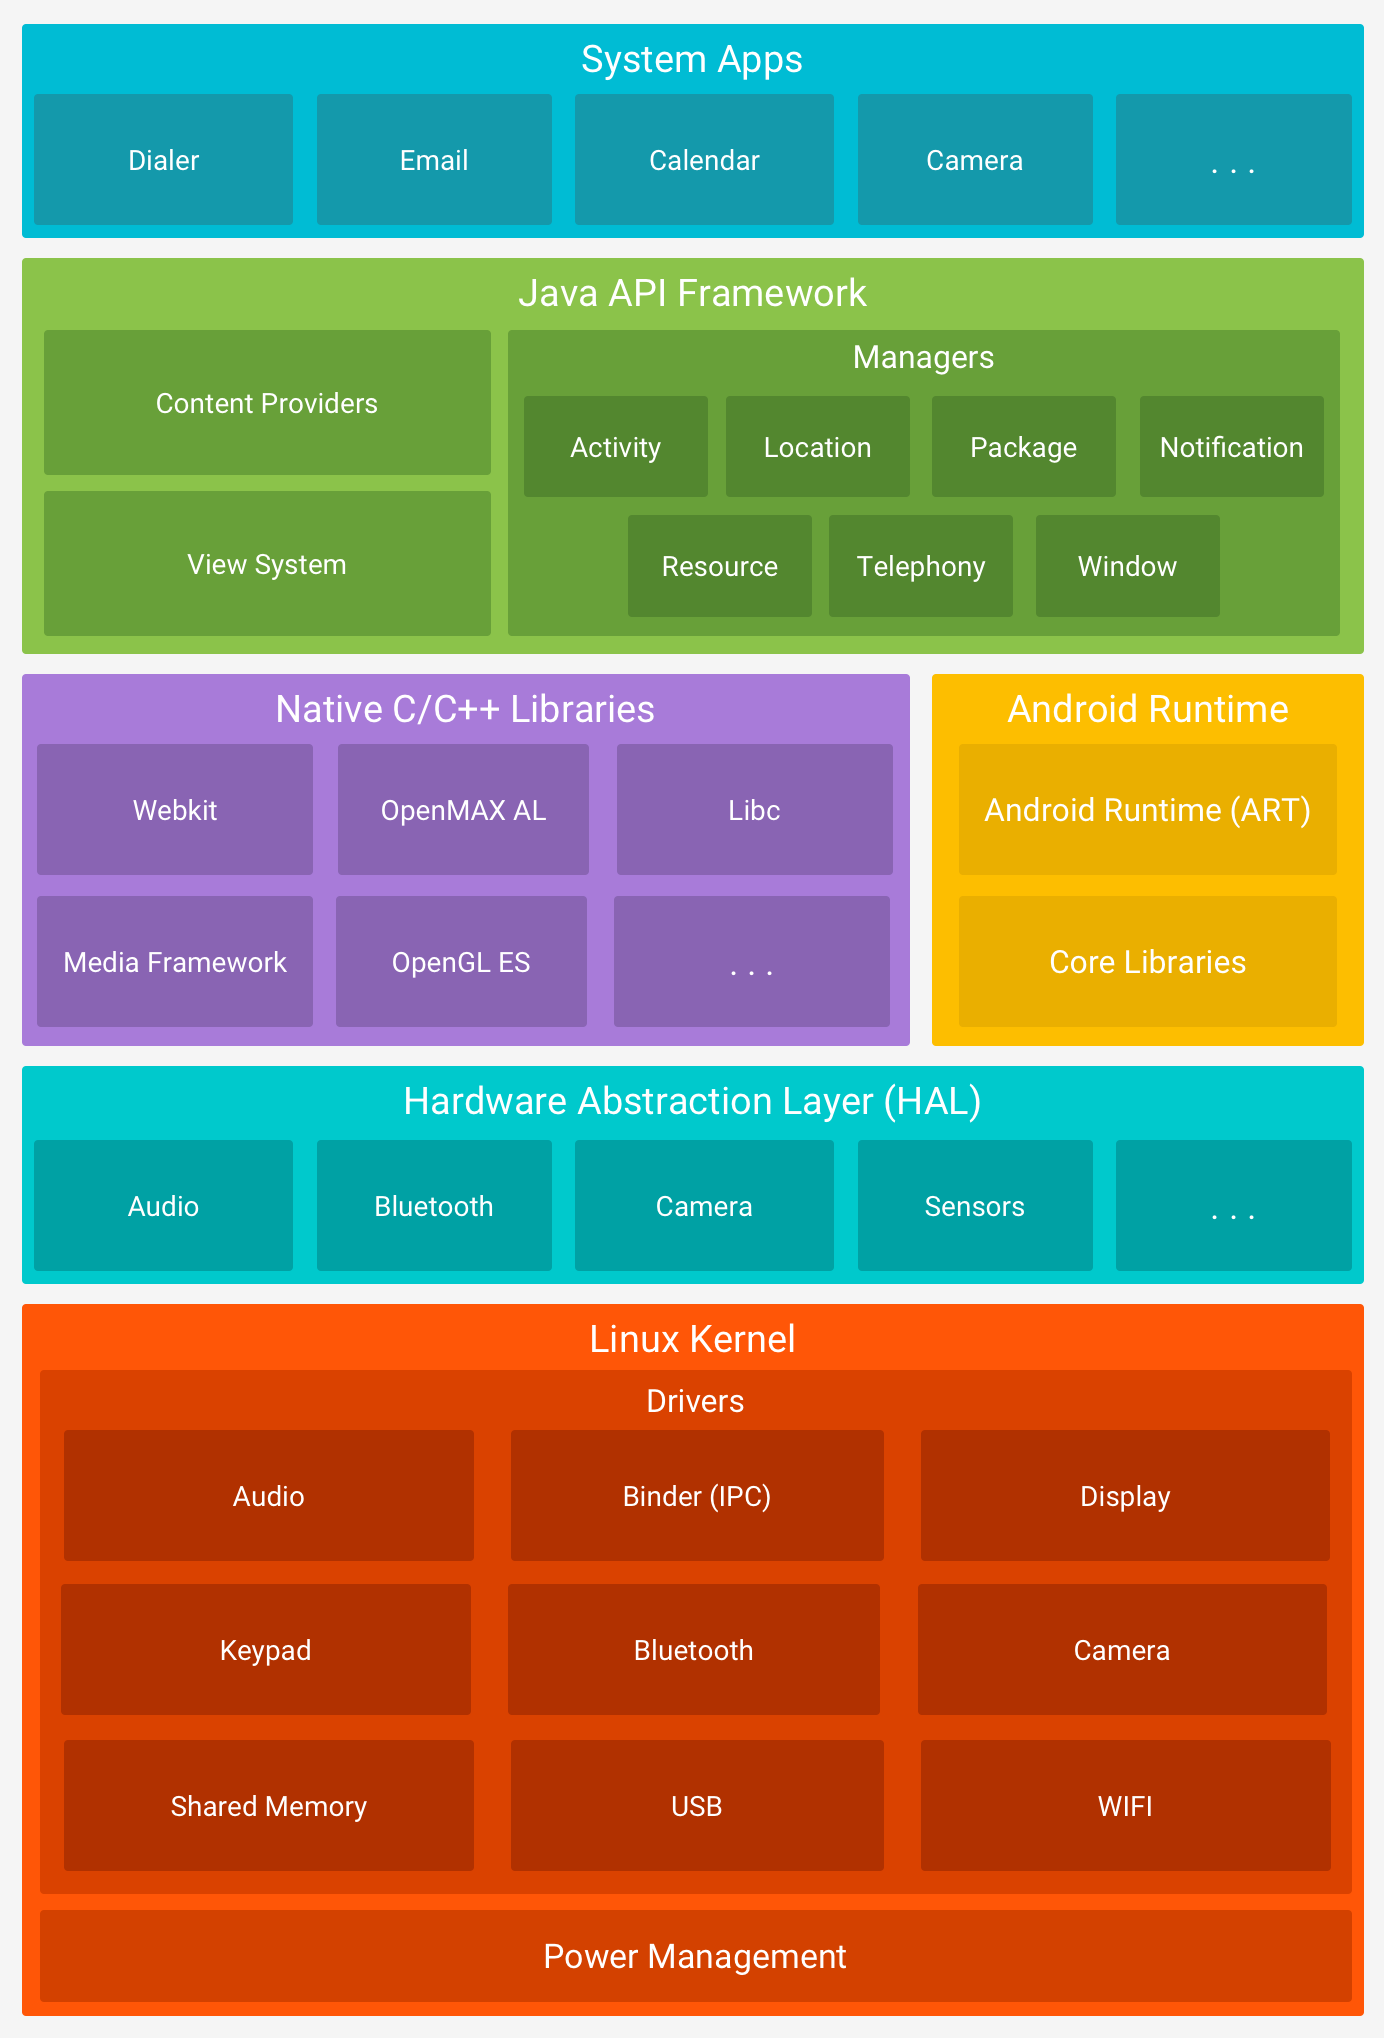
\includegraphics[scale=0.09]{../imagenes/android-stack.png}
            \end{figure}
        \end{column}
    \end{columns}
\end{frame}


\begin{frame}{Ejemplo de la propiedad II}
    \begin{enumerate}[<+->]
        \item Una aplicación $A$ declara el permiso $P$ agrupado en el grupo $G$
        \item Una aplicación $B$ solicita el permiso $P$
        \item El usuario otorga el permiso $P$ a la aplicación $B$
        \item La aplicación $A$ se desinstala (y por lo tanto los permisos declarados por ella son
              eliminados)
        \item La aplicación $B$ puede otorgar automáticamente los permisos pertenecientes al grupo $G$
              (a pesar de que ya no cuenta con el permiso $P$)
    \end{enumerate}
\end{frame}

\begin{frame}{Todas las acciones}{Parte I}
    \fontsize{8pt}{9pt}\selectfont
    \begin{table}
        \begin{tabularx}{\linewidth}{|l X|}
            \hline
            \textbf{Acción}                    & \textbf{Descripción}                                                                                                                                               \\
            \hline
            $\mathtt{install}~app~m~c~res$     & Instala la aplicación con identificador $app$, cuyo manifiesto es $m$, su certificado es $c$ y la lista de recursos es $res$.                                      \\
            \hline
            $\mathtt{uninstall}~app$           & Desinstala la aplicación con identificador $app$.                                                                                                                  \\
            \hline
            $\mathtt{read}~ic~cp~u$            & El componente en ejecución $ic$ lee el recurso correspondiente al identificador URI $u$ del proveedor de contenido $cp$.                                           \\
            \hline
            $\mathtt{write}~ic~cp~u~val$       & El componente en ejecución $ic$ escribe el valor $val$ en el recurso correspondiente al identificador $u$ del proveedor de contenido $cp$.                         \\
            \hline
            $\mathtt{startActivity}~i~ic$      & El componente en ejecución $ic$ solicita comenzar la actividad especificada por el intent $i$.                                                                     \\
            \hline
            $\mathtt{startActivityRes}~i~n~ic$ & El componente en ejecución $ic$ solicita comenzar la actividad especificada por el intent $i$ y espera como respuesta un token $n$.                                \\
            \hline
            $\mathtt{startService}~i~ic$       & El componente en ejecución $ic$ solicita comenzar el servicio especificado por el intent $i$.                                                                      \\
            \hline
            $\mathtt{sendBroadcast}~i~ic~p$    & El componente en ejecución $ic$ envía el intent $i$ en modo \textit{broadcast}, especificando que solo los componentes que posean el permiso $p$ pueden recibirlo. \\
            \hline
        \end{tabularx}
    \end{table}
\end{frame}

\begin{frame}{Todas las acciones}{Parte II}
    \fontsize{9pt}{10pt}\selectfont
    \begin{table}
        \begin{tabularx}{\linewidth}{|l X|}
            \hline
            \textbf{Acción}                    & \textbf{Descripción}                                                                                                                                                                                                 \\
            \hline
            $\mathtt{sendOrdBroadcast}~i~ic~p$ & El componente en ejecución $ic$ envía el intent $i$ en modo \textit{broadcast} ordenado,  especificando que solo los componentes que posean el permiso $p$ pueden recibirlo.                                         \\
            \hline
            $\mathtt{sendSBroadcast}~i~ic$     & El componente en ejecución $ic$ envía el intent $i$ en modo \textit{sticky broadcast}.                                                                                                                               \\
            \hline
            $\mathtt{resolveIntent}~i~app$     & La aplicación $app$ vuelve al intent $i$ explícito.                                                                                                                                                                  \\
            \hline
            $\mathtt{stop}~ic$                 & El componente en ejecución $ic$ termina su ejecución.                                                                                                                                                                \\
            \hline
            $\mathtt{grantP}~ic~cp~app~u~op$   & El componente en ejecución $ic$ delega permisos permantentes a la aplicación $app$. Esta delegación autoriza a $app$ a realizar la operación $op$ en el recurso asignado al URI $u$ del proveedor de contenido $cp$. \\
            \hline
            $\mathtt{revokeDel}~ic~cp~u~op$    & El componente en ejecución $ic$ revoca los permisos otorgados al recurso $u$ del proveedor de contenidos $cp$ para realizar la operación $op$.                                                                       \\
            \hline
            $\mathtt{call}~ic~sac$             & El componente en ejecución $ic$ realiza el llamado a una función del sistema denominada $sac$.                                                                                                                       \\
            \hline
        \end{tabularx}
    \end{table}
\end{frame}

\begin{frame}{Todas las acciones}{Parte III}
    \fontsize{9pt}{11pt}\selectfont
    \begin{table}
        \begin{tabularx}{\linewidth}{|l X|}
            \hline
            \textbf{Acción}                   & \textbf{Descripción}                                                                                                                                                                   \\
            \hline
            $\mathtt{grant}~p~app$            & Otorga el permiso $p$ a la aplicación $app$ con la confirmación del usuario.                                                                                                           \\
            \hline
            $\mathtt{grantAuto}~p~app$        & Otorga automáticamente el permiso $p$ a la aplicación $app$ (sin requerir confirmación del usuario).                                                                                   \\
            \hline
            $\mathtt{revoke}~p~app$           & Revoca un permiso no agrupado $p$ de la aplicación $app$.                                                                                                                              \\
            \hline
            $\mathtt{revokePermGroup}~g~app$  & Revoca todos los permisos pertenecientes al grupo $g$ de la aplicación $app$.                                                                                                          \\
            \hline
            $\mathtt{hasPermission}~p~app$    & Chequea si la aplicación $app$ posee el permiso $p$.                                                                                                                                   \\
            \hline
            $\mathtt{receiveIntent}~i~ic~app$ & La aplicación $app$ recibe el intent $i$, enviado por el componente en ejecución $ic$.                                                                                                 \\
            \hline
            $\mathtt{verifyOldApp}~app$       & El usuario verifica los permisos que han sido otorgados a la aplicación $app$. Solo se utiliza para aquellas aplicaciones que fueron instaladas previamente a la versión 6 de Android. \\
            \hline
        \end{tabularx}
    \end{table}
\end{frame}
\end{document}